\documentclass[convert]{standalone}
\usepackage{tikz}

\begin{document}
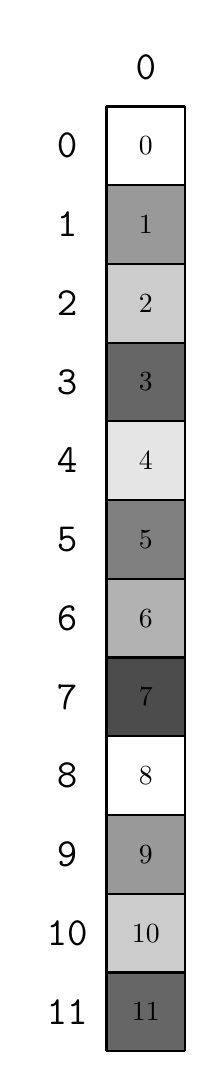
\begin{tikzpicture}[x={(0cm,-1cm)},y={(1cm,0cm)},every node/.style={minimum size=1cm, outer sep=0pt}]

\node[fill=black!00] at (0,0) {0};
\node[fill=black!40] at (1,0) {1};
\node[fill=black!20] at (2,0) {2};
\node[fill=black!60] at (3,0) {3};
\node[fill=black!10] at (4,0) {4};
\node[fill=black!50] at (5,0) {5};
\node[fill=black!30] at (6,0) {6};
\node[fill=black!70] at (7,0) {7};
\node[fill=black!00] at (8,0) {8};
\node[fill=black!40] at (9,0) {9};
\node[fill=black!20] at (10,0) {10};
\node[fill=black!60] at (11,0) {11};
\draw[color=black,thick,shift={(-0.5,-0.5)}] (0,0) grid (12,1);

\node at (0,-1) {\Large{\texttt{0}}};
\node at (1,-1) {\Large{\texttt{1}}};
\node at (2,-1) {\Large{\texttt{2}}};
\node at (3,-1) {\Large{\texttt{3}}};
\node at (4,-1) {\Large{\texttt{4}}};
\node at (5,-1) {\Large{\texttt{5}}};
\node at (6,-1) {\Large{\texttt{6}}};
\node at (7,-1) {\Large{\texttt{7}}};
\node at (8,-1) {\Large{\texttt{8}}};
\node at (9,-1) {\Large{\texttt{9}}};
\node at (10,-1) {\Large{\texttt{10}}};
\node at (11,-1) {\Large{\texttt{11}}};
\node at (-1,0) {\Large{\texttt{0}}};
\end{tikzpicture}
\end{document}